\documentclass[journal,12pt,twocolumn]{IEEEtran}

\usepackage{setspace}
\usepackage{gensymb}
\singlespacing
\usepackage[cmex10]{amsmath}

\usepackage{amsthm}

\usepackage{mathrsfs}
\usepackage{txfonts}
\usepackage{stfloats}
\usepackage{bm}
\usepackage{cite}
\usepackage{cases}
\usepackage{subfig}

\usepackage{longtable}
\usepackage{multirow}

\usepackage{enumitem}
\usepackage{mathtools}
\usepackage{steinmetz}
\usepackage{tikz}
\usepackage{circuitikz}
\usepackage{verbatim}
\usepackage{tfrupee}
\usepackage[breaklinks=true]{hyperref}
\usepackage{graphicx}
\usepackage{tkz-euclide}

\usetikzlibrary{calc,math}
\usepackage{listings}
    \usepackage{color}                                            %%
    \usepackage{array}                                            %%
    \usepackage{longtable}                                        %%
    \usepackage{calc}                                             %%
    \usepackage{multirow}                                         %%
    \usepackage{hhline}                                           %%
    \usepackage{ifthen}                                           %%
    \usepackage{lscape}     
\usepackage{multicol}
\usepackage{chngcntr}

\DeclareMathOperator*{\Res}{Res}

\renewcommand\thesection{\arabic{section}}
\renewcommand\thesubsection{\thesection.\arabic{subsection}}
\renewcommand\thesubsubsection{\thesubsection.\arabic{subsubsection}}

\renewcommand\thesectiondis{\arabic{section}}
\renewcommand\thesubsectiondis{\thesectiondis.\arabic{subsection}}
\renewcommand\thesubsubsectiondis{\thesubsectiondis.\arabic{sub subsection}}


\hyphenation{optical networks semiconduc-tor}
\def\inputGnumericTable{}                                 %%

\lstset{
%language=C,
frame=single, 
breaklines=true,
columns=fullflexible
}
\date{March 2021}

\begin{document}

\newcommand{\BEQA}{\begin{eqnarray}}
\newcommand{\EEQA}{\end{eqnarray}}
\newcommand{\define}{\stackrel{\triangle}{=}}
\bibliographystyle{IEEEtran}
\raggedbottom
\setlength{\parindent}{0pt}
\providecommand{\mbf}{\mathbf}
\providecommand{\pr}[1]{\ensuremath{\Pr\left(#1\right)}}
\providecommand{\qfunc}[1]{\ensuremath{Q\left(#1\right)}}
\providecommand{\fn}[1]{\ensuremath{f\left(#1\right)}}
\providecommand{\e}[1]{\ensuremath{E\left(#1\right)}}
\providecommand{\sbrak}[1]{\ensuremath{{}\left[#1\right]}}
\providecommand{\lsbrak}[1]{\ensuremath{{}\left[#1\right.}}
\providecommand{\rsbrak}[1]{\ensuremath{{}\left.#1\right]}}
\providecommand{\brak}[1]{\ensuremath{\left(#1\right)}}
\providecommand{\lbrak}[1]{\ensuremath{\left(#1\right.}}
\providecommand{\rbrak}[1]{\ensuremath{\left.#1\right)}}
\providecommand{\cbrak}[1]{\ensuremath{\left\{#1\right\}}}
\providecommand{\lcbrak}[1]{\ensuremath{\left\{#1\right.}}
\providecommand{\rcbrak}[1]{\ensuremath{\left.#1\right\}}}
\theoremstyle{remark}
\newtheorem{rem}{Remark}
\newcommand{\sgn}{\mathop{\mathrm{sgn}}}
\providecommand{\abs}[1]{\vert#1\vert}
\providecommand{\res}[1]{\Res\displaylimits_{#1}} 
\providecommand{\norm}[1]{\lVert#1\rVert}
%\providecommand{\norm}[1]{\lVert#1\rVert}
\providecommand{\mtx}[1]{\mathbf{#1}}
\providecommand{\mean}[1]{E[ #1 ]}
\providecommand{\fourier}{\overset{\mathcal{F}}{ \rightleftharpoons}}
%\providecommand{\hilbert}{\overset{\mathcal{H}}{ \rightleftharpoons}}
\providecommand{\system}{\overset{\mathcal{H}}{ \longleftrightarrow}}
	%\newcommand{\solution}[2]{\textbf{Solution:}{#1}}
\newcommand{\solution}{\noindent \textbf{Solution: }}
\newcommand{\cosec}{\,\text{cosec}\,}
\providecommand{\dec}[2]{\ensuremath{\overset{#1}{\underset{#2}{\gtrless}}}}
\newcommand{\myvec}[1]{\ensuremath{\begin{pmatrix}#1\end{pmatrix}}}
\newcommand{\mydet}[1]{\ensuremath{\begin{vmatrix}#1\end{vmatrix}}}
\numberwithin{equation}{subsection}
\makeatletter
\@addtoreset{figure}{problem}
\makeatother
\let\StandardTheFigure\thefigure
\let\vec\mathbf
\renewcommand{\thefigure}{\theproblem}
\def\putbox#1#2#3{\makebox[0in][l]{\makebox[#1][l]{}\raisebox{\baselineskip}[0in][0in]{\raisebox{#2}[0in][0in]{#3}}}}
     \def\rightbox#1{\makebox[0in][r]{#1}}
     \def\centbox#1{\makebox[0in]{#1}}
     \def\topbox#1{\raisebox{-\baselineskip}[0in][0in]{#1}}
     \def\midbox#1{\raisebox{-0.5\baselineskip}[0in][0in]{#1}}
\vspace{3cm}
\title{ AI1103 : Assignment-2}
\author{Nelakuditi Rahul Naga - AI20BTECH11029/EE20BTECH11036}
\maketitle
\newpage
\bigskip
\renewcommand{\thefigure}{\theenumi}
\renewcommand{\thetable}{\theenumi}

Download all python codes from 
\begin{lstlisting}
https://github.com/Rahul27n/Assignment_2/blob/main/Assignment_2.py
\end{lstlisting}
%
and latex-tikz codes from 
%
\begin{lstlisting}
https://github.com/Rahul27n/Assignment_2/blob/main/Assignment_2.tex
\end{lstlisting}
\vspace{0.5cm}
\section{QUESTION: Q.33 EE-GATE-2016-SET-2}
\vspace{0.5cm}

Let the probability density function of random variable,$X$,be given as:\\
\\$f_x(x)$ = $\frac{3}{2}$$e^{-3x}$${u(x)}$ + $a$$e^{4x}$${u(-x)}$\\
\\where u(x) is the unit step function.Then the value of a and Prob\{$X\leq0$\}, respectively,are:\\
\\(A) 2,$\frac{1}{2}$\\
\\(B) 4,$\frac{1}{2}$\\
\\(C) 2,$\frac{1}{4}$\\
\\(D) 4,$\frac{1}{4}$\\

\section{SOLUTION:}
\vspace{0.5cm}

We know that,
\begin{align}
\int_{-\infty}^{\infty}{f_x(x)}\,dx = 1.\\
\int_{-\infty}^{0}{f_x(x)}\,dx +\int_{0}^{\infty}{f_x(x)}\,dx = 1\label{eq_(1)}\\
\int_{-\infty}^{0}{ae^{4x}}\,dx +\int_{0}^{\infty}{\frac{3}{2}e^{-3x}}\,dx = 1\label{eq_(2)}
\end{align}
The expression \eqref{eq_(2)} was written from \eqref{eq_(1)} since,
\begin{align*}
  u(x) = 
  \begin{cases}
  1, & \text{for } x \geq 0\\
  0, & \text{otherwise } 
  \end{cases}
\end{align*}

Simplifying \eqref{eq_(2)} we have:
\begin{align}
\int_{-\infty}^{0}{ae^{4x}}\,dx +\int_{0}^{\infty}{\frac{3}{2}e^{-3x}}\,dx = 1\nonumber\\
\implies a\left[\frac{e^{4x}}{4}\right]_{-\infty}^{0} +    \frac{3}{2}\left[\frac{e^{-3x}}{-3}\right]_0^{\infty} = 1\\
\implies a\left[\frac{1}{4}-0\right] - \frac{1}{2}\left[0-1\right] = 1\\
\implies \frac{a}{4} + \frac{1}{2} =1 \implies a = 2
\end{align}
Therefore,
\begin{align}
 f_x(x) = 
  \begin{cases}
  \frac{3}{2}e^{-3x}, & \text{for } x \geq 0\\
  2e^{4x}, & \text{for } x < 0
  \end{cases}
\end{align}

The plot for PDF of $X$ can be observed at figure \ref{fig:The PDF of X}
\begin{figure}[!ht]
       \centering
    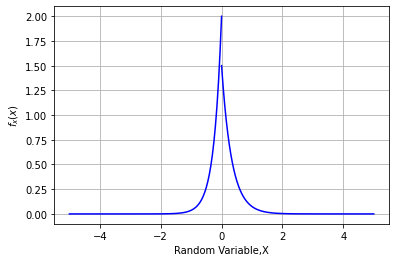
\includegraphics[width=.9\columnwidth] {Assignment_2_Fig_2.png}
    \caption{The PDF of X}
    \label{fig:The PDF of X}
\end{figure}

The CDF of X is defined as follows:
\begin{align}
    F_X(x)= \pr{X\leq x}
\end{align}
Now for $x<0$,
\begin{align}
\pr{X\leq x} &= \int_{-\infty}^{x}{f_x(x)}\,dx\\
&= \int_{-\infty}^{x}{2e^{4x}}\,dx\\
&= 2\left[\frac{e^{4x}}{4}\right]_{-\infty}^{x}\\
&= 2\left[\frac{e^{4x}}{4}-0\right]\\
&= \frac{e^{4x}}{2}
\end{align}
Similarly for $x\geq0$,
\begin{align}
\pr{X\leq x} &= \int_{-\infty}^{x}{f_x(x)}\,dx\\
&= \int_{-\infty}^{0}{2e^{4x}}\,dx +\int_{0}^{x}{\frac{3}{2}e^{-3x}}\,dx\\
&= 2\left[\frac{e^{4x}}{4}\right]_{-\infty}^{0}+\left[\frac{-e^{-3x}}{2}\right]_{0}^{x}\\
&= 2\left[\frac{1}{4}-0\right]-\frac{1}{2}\left[e^{-3x}-1\right]\\
&= 1-\frac{e^{-3x}}{2}
\end{align}

The CDF of X is as below:
\begin{align}
 F_X(x) = 
  \begin{cases}
  1-\frac{e^{-3x}}{2}, & \text{for } x \geq 0\\
  \frac{e^{4x}}{2}, & \text{for } x < 0
  \end{cases}
\end{align}

The plot for CDF of $X$ can be observed at figure \ref{fig:The PDF of X}.
\begin{figure}[!ht]
       \centering
    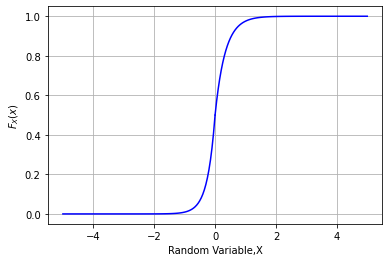
\includegraphics[width=.9\columnwidth] {Assignment_2_Fig_1.png}
    \caption{The CDF of X}
    \label{fig:The CDF of X}
\end{figure}

\begin{align}
\therefore
\pr{X\leq0} = F_X(0)=\frac{1}{2}
\end{align}
Hence the correct answer is option (A).

\end{document}